\begin{figure}[h!]
	\centering
	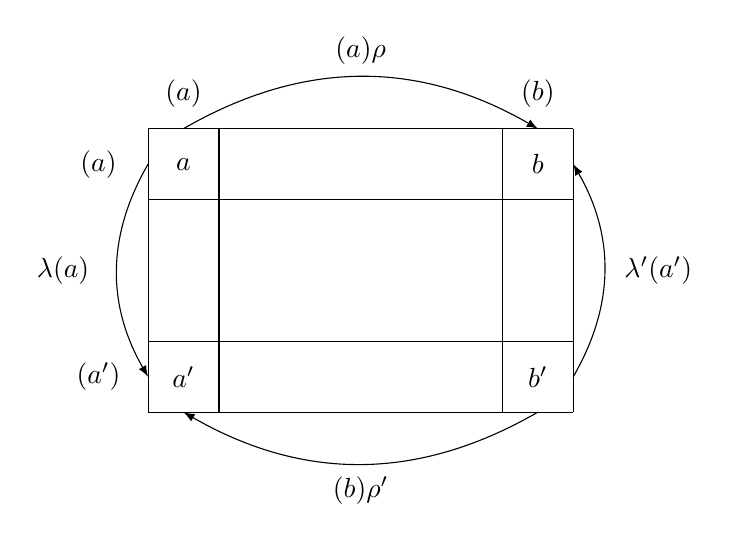
\begin{tikzpicture}[scale = 0.9]
	\tikzstyle{fleche}=[->,>=latex,rounded corners=4pt]
	\node at (0,0){$a'$};
	\node at (0,3){$a$};
	\node at (5,0){$b'$};
	\node at (5,3){$b$};
	\draw (-.5,3.5) -- (-.5, -.5);
	\draw (.5,3.5) -- (.5, -.5);
	\draw (5.5,3.5) -- (5.5, -.5);
	\draw (4.5,3.5) -- (4.5, -.5);
	\draw (-.5,3.5) -- (5.5, 3.5);
	\draw (-.5,2.5) -- (5.5, 2.5);
	\draw (-.5,.5) -- (5.5, .5);
	\draw (-.5,-.5) -- (5.5, -.5);
	
	\draw[->, >=latex, bend right] (-.5,3) to (-.5,0);
	\node at (-1.7, 1.5){$\lambda\mul{\rc(a)}$};
	\draw[->, >=latex, bend right] (5.5,0) to (5.5,3);
	\node at (6.7, 1.5){$\lambda'\mul{\rc(a')}$};
	\draw[->, >=latex, bend left] (0,3.5) to (5,3.5);
	\node at (2.5, 4.6){$\mul{\lc(a)}\rho$};
	\draw[->, >=latex, bend left] (5,-.5) to (0,-.5);
	\node at (2.5, -1.6){$\mul{\lc(b)}\rho'$};
	
	\node at (-1.2, 3){$\rc(a)$};
	\node at (-1.2, 0){$\rc(a')$};
	\node at (0, 4){$\lc(a)$};
	\node at (5, 4){$\lc(b)$};
	
	\end{tikzpicture}
	\caption{Green's Lemma}
\end{figure}